\documentclass[../manuale-sviluppatore.tex]{subfiles}

\begin{document}

\subsection{Server}%
\label{sub:server}

Il backend di Stalker è costituito da un server scritto in linguaggio Java e realizzato tramite il framework \glossario{Spring Webflux}.
Il suo compito principale è quello di  soddisfare le richieste dei client che avvengono tramite chiamate di rete Http, gestire la logica di business e manipolare i modelli di dati.
Il server, inoltre, implementa gli endpoints definiti all'interno dell'\glossario{API}.

\subsubsection{Architettura backend}%
\label{architettura_backend}

L'architettura del backend, che ci è stata fortemente suggerita dal framework Spring, è monolitica.
Essa è suddivisa in strati che svolgono una funzione definita e hanno un ruolo ben distinto.
Più nello specifico, il server di Stalker ha un' architettura monolitica organizzata in 5 layer che sono così denominati:
\begin{itemize}
  \item Controller
  \item Service
  \item Model
  \item Repository
  \item Database
\end{itemize}

\begin{figure}[H]
  \centering
  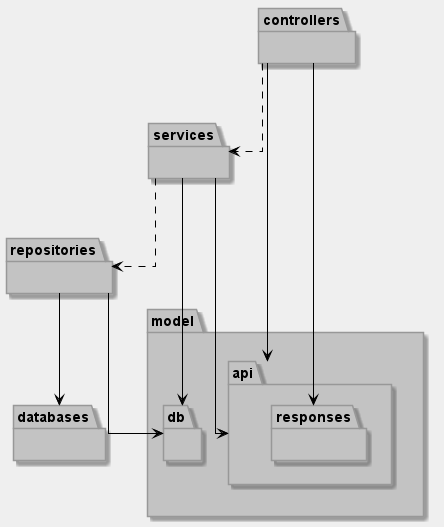
\includegraphics[width=10cm, height=8cm]{img/server-package-diagram.png}
  \caption{Diagramma dei package che illustra la struttura del server}%
   \label{fig:diagramma dei package che illustra la struttura del server}
\end{figure}

Per soddisfare le richieste dei client, le informazioni devono passare attraverso tutti gli strati.
Il controller è il layer più superficiale e che si interfaccia con le altre componenti.
Esso, inoltra la richiesta agli strati sottostanti fino allo strato di persistenza dove il server cercherà di soddisfarla.
Sia in caso di successo che di errore il server risponderà con un codice di stato Http.

Segue ora una breve descrizione dei compiti di ogni strato.

\subsubsection{Controller}%
\label{subs:controller}

Il controller è lo strato del server che si interfaccia direttamente con i client.
Ogniqualvolta una richiesta di un client arriva al server una funzione di un controller sarà incaricata di soddisfarla.
Ciò in spring avviene grazie a delle annotazioni che effettuano il mapping tra l'endpoint e la funzione che svolgerà il ruolo di handler.

\begin{figure}[H]
  \centering
  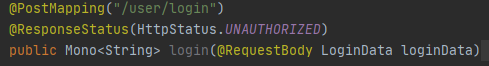
\includegraphics{img/controller-image.png}
  \caption{Immagine che illustra un endpoint di esempio}%
   \label{fig:immagine che illustra un endpoint di esempio}
\end{figure}

Nell'immagine soprastante si può osservare un esempio di handler implementato nel controller.
L'annotazione \textit{@PostMapping} indica che la funzione si attiverà nel caso di una chiamata post all'endpoint /user/login.
È presente, inoltre, l'annotazione \textit{@ResponseStatus} che stabilisce il tipo di codice di stato http che verrà restituito nel caso in cui la chiamata andasse a buon fine.

\end{document}
